% Options for packages loaded elsewhere
\PassOptionsToPackage{unicode}{hyperref}
\PassOptionsToPackage{hyphens}{url}
\PassOptionsToPackage{dvipsnames,svgnames,x11names}{xcolor}
%
\documentclass[
  letterpaper,
  DIV=11,
  numbers=noendperiod]{scrartcl}

\usepackage{amsmath,amssymb}
\usepackage{iftex}
\ifPDFTeX
  \usepackage[T1]{fontenc}
  \usepackage[utf8]{inputenc}
  \usepackage{textcomp} % provide euro and other symbols
\else % if luatex or xetex
  \usepackage{unicode-math}
  \defaultfontfeatures{Scale=MatchLowercase}
  \defaultfontfeatures[\rmfamily]{Ligatures=TeX,Scale=1}
\fi
\usepackage{lmodern}
\ifPDFTeX\else  
    % xetex/luatex font selection
\fi
% Use upquote if available, for straight quotes in verbatim environments
\IfFileExists{upquote.sty}{\usepackage{upquote}}{}
\IfFileExists{microtype.sty}{% use microtype if available
  \usepackage[]{microtype}
  \UseMicrotypeSet[protrusion]{basicmath} % disable protrusion for tt fonts
}{}
\makeatletter
\@ifundefined{KOMAClassName}{% if non-KOMA class
  \IfFileExists{parskip.sty}{%
    \usepackage{parskip}
  }{% else
    \setlength{\parindent}{0pt}
    \setlength{\parskip}{6pt plus 2pt minus 1pt}}
}{% if KOMA class
  \KOMAoptions{parskip=half}}
\makeatother
\usepackage{xcolor}
\setlength{\emergencystretch}{3em} % prevent overfull lines
\setcounter{secnumdepth}{5}
% Make \paragraph and \subparagraph free-standing
\ifx\paragraph\undefined\else
  \let\oldparagraph\paragraph
  \renewcommand{\paragraph}[1]{\oldparagraph{#1}\mbox{}}
\fi
\ifx\subparagraph\undefined\else
  \let\oldsubparagraph\subparagraph
  \renewcommand{\subparagraph}[1]{\oldsubparagraph{#1}\mbox{}}
\fi


\providecommand{\tightlist}{%
  \setlength{\itemsep}{0pt}\setlength{\parskip}{0pt}}\usepackage{longtable,booktabs,array}
\usepackage{calc} % for calculating minipage widths
% Correct order of tables after \paragraph or \subparagraph
\usepackage{etoolbox}
\makeatletter
\patchcmd\longtable{\par}{\if@noskipsec\mbox{}\fi\par}{}{}
\makeatother
% Allow footnotes in longtable head/foot
\IfFileExists{footnotehyper.sty}{\usepackage{footnotehyper}}{\usepackage{footnote}}
\makesavenoteenv{longtable}
\usepackage{graphicx}
\makeatletter
\def\maxwidth{\ifdim\Gin@nat@width>\linewidth\linewidth\else\Gin@nat@width\fi}
\def\maxheight{\ifdim\Gin@nat@height>\textheight\textheight\else\Gin@nat@height\fi}
\makeatother
% Scale images if necessary, so that they will not overflow the page
% margins by default, and it is still possible to overwrite the defaults
% using explicit options in \includegraphics[width, height, ...]{}
\setkeys{Gin}{width=\maxwidth,height=\maxheight,keepaspectratio}
% Set default figure placement to htbp
\makeatletter
\def\fps@figure{htbp}
\makeatother
% definitions for citeproc citations
\NewDocumentCommand\citeproctext{}{}
\NewDocumentCommand\citeproc{mm}{%
  \begingroup\def\citeproctext{#2}\cite{#1}\endgroup}
\makeatletter
 % allow citations to break across lines
 \let\@cite@ofmt\@firstofone
 % avoid brackets around text for \cite:
 \def\@biblabel#1{}
 \def\@cite#1#2{{#1\if@tempswa , #2\fi}}
\makeatother
\newlength{\cslhangindent}
\setlength{\cslhangindent}{1.5em}
\newlength{\csllabelwidth}
\setlength{\csllabelwidth}{3em}
\newenvironment{CSLReferences}[2] % #1 hanging-indent, #2 entry-spacing
 {\begin{list}{}{%
  \setlength{\itemindent}{0pt}
  \setlength{\leftmargin}{0pt}
  \setlength{\parsep}{0pt}
  % turn on hanging indent if param 1 is 1
  \ifodd #1
   \setlength{\leftmargin}{\cslhangindent}
   \setlength{\itemindent}{-1\cslhangindent}
  \fi
  % set entry spacing
  \setlength{\itemsep}{#2\baselineskip}}}
 {\end{list}}
\usepackage{calc}
\newcommand{\CSLBlock}[1]{\hfill\break\parbox[t]{\linewidth}{\strut\ignorespaces#1\strut}}
\newcommand{\CSLLeftMargin}[1]{\parbox[t]{\csllabelwidth}{\strut#1\strut}}
\newcommand{\CSLRightInline}[1]{\parbox[t]{\linewidth - \csllabelwidth}{\strut#1\strut}}
\newcommand{\CSLIndent}[1]{\hspace{\cslhangindent}#1}

\usepackage{booktabs}
\usepackage{longtable}
\usepackage{array}
\usepackage{multirow}
\usepackage{wrapfig}
\usepackage{float}
\usepackage{colortbl}
\usepackage{pdflscape}
\usepackage{tabu}
\usepackage{threeparttable}
\usepackage{threeparttablex}
\usepackage[normalem]{ulem}
\usepackage{makecell}
\usepackage{xcolor}
\usepackage{siunitx}

  \newcolumntype{d}{S[
    input-open-uncertainty=,
    input-close-uncertainty=,
    parse-numbers = false,
    table-align-text-pre=false,
    table-align-text-post=false
  ]}
  
\KOMAoption{captions}{tableheading}
\makeatletter
\@ifpackageloaded{caption}{}{\usepackage{caption}}
\AtBeginDocument{%
\ifdefined\contentsname
  \renewcommand*\contentsname{Table of contents}
\else
  \newcommand\contentsname{Table of contents}
\fi
\ifdefined\listfigurename
  \renewcommand*\listfigurename{List of Figures}
\else
  \newcommand\listfigurename{List of Figures}
\fi
\ifdefined\listtablename
  \renewcommand*\listtablename{List of Tables}
\else
  \newcommand\listtablename{List of Tables}
\fi
\ifdefined\figurename
  \renewcommand*\figurename{Figure}
\else
  \newcommand\figurename{Figure}
\fi
\ifdefined\tablename
  \renewcommand*\tablename{Table}
\else
  \newcommand\tablename{Table}
\fi
}
\@ifpackageloaded{float}{}{\usepackage{float}}
\floatstyle{ruled}
\@ifundefined{c@chapter}{\newfloat{codelisting}{h}{lop}}{\newfloat{codelisting}{h}{lop}[chapter]}
\floatname{codelisting}{Listing}
\newcommand*\listoflistings{\listof{codelisting}{List of Listings}}
\makeatother
\makeatletter
\makeatother
\makeatletter
\@ifpackageloaded{caption}{}{\usepackage{caption}}
\@ifpackageloaded{subcaption}{}{\usepackage{subcaption}}
\makeatother
\ifLuaTeX
  \usepackage{selnolig}  % disable illegal ligatures
\fi
\usepackage{bookmark}

\IfFileExists{xurl.sty}{\usepackage{xurl}}{} % add URL line breaks if available
\urlstyle{same} % disable monospaced font for URLs
\hypersetup{
  pdftitle={Respiratory-Related Mortality Rates Show A Positive Correlation With Increasing Air pollution},
  pdfauthor={Vanshika Vanshika; Shivank Goel; Navya Hooda},
  colorlinks=true,
  linkcolor={blue},
  filecolor={Maroon},
  citecolor={Blue},
  urlcolor={Blue},
  pdfcreator={LaTeX via pandoc}}

\title{Respiratory-Related Mortality Rates Show A Positive Correlation
With Increasing Air pollution\thanks{Code and data are available at:
https://github.com/shivankgoel003/Mortality-in-Alberta.}}
\usepackage{etoolbox}
\makeatletter
\providecommand{\subtitle}[1]{% add subtitle to \maketitle
  \apptocmd{\@title}{\par {\large #1 \par}}{}{}
}
\makeatother
\subtitle{Based on Data Collected From The Province Of Alberta}
\author{Vanshika Vanshika \and Shivank Goel \and Navya Hooda}
\date{March 15, 2024}

\begin{document}
\maketitle
\begin{abstract}
First sentence. Second sentence. Third sentence. Fourth sentence.
\end{abstract}

\section{Introduction}\label{introduction}

The impact of air pollution on human health has increasingly become a
global concern, with respiratory illnesses being a significant
consequence of poor air quality. The National Library of Medicine
reports that approximately 4 million people die prematurely each year
from chronic respiratory diseases linked to air pollution Med (2020).
The World Health Organization also suggests that air pollution poses a
risk for all-cause mortality and specific diseases, especially the
exposure to air pollution is strongly linked with outcomes such as
stroke, ischemic heart disease, chronic obstructive pulmonary disease,
lung cancer, pneumonia, and cataracts Organization (2024).

The pollutants most significantly concerning for public health, are
particulate matter (PM), carbon monoxide (CO), ozone (O3), nitrogen
dioxide (NO2), and sulfur dioxide (SO2). Of these, fine particulate
matter is particularly worrisome due to its ability to penetrate the
lungs deeply, enter the bloodstream, and reach organs, leading to
systemic damage to tissues and cells.

Specifically, PM2.5 is of greater concern due to its harmful properties
and dangers. PM2.5 is airborne particulate matter (PM2.5) and is not a
single pollutant but rather a mixture of many chemical species and
aerosols. PM2.5 is associated with the greatest proportion of adverse
health effects related to air pollution, both in the United States and
worldwide. Long-term (months to years) exposure to PM2.5 has been linked
to premature death, particularly in people who have chronic heart or
lung diseases, and reduced lung function growth in children Board
(2024).

In this paper, we analyze data from Alberta, Canada, and aim to explore
the estimand of the number of deaths that can be correlated to the Air
Quality Health Index (AQHI) and PM2.5 quantities. Specifically, we
assess how AQHI relates to the prevalence of respiratory and cardiac
illnesses in this specific region, focusing on four major types: Chronic
Obstructive Pulmonary Disease, Ischemic Heart Disease, Acute Myocardial
Infarction, and Lung Cancer. We use the mortality rate in Alberta data
to select respiratory-related illnesses and air quality health index
data for Alberta through their provincial open data portal. To analyze
respiratory illnesses, we use air pollution measured through the AQHI
and specifically the particulate matter 2.5 (PM2.5) air pollutant as a
predictor of mortality related to respiratory illnesses. In total, we
will be assessing the overall relationship between AQHI and respiratory
illnesses, the relationship between PM2.5 and respiratory illnesses, as
well as the relevance of PM2.5 levels in lung and heart disease values
as a means to draw any notable significance of PM2.5 in different types
of illnesses.

Using negative binomial regression, this study seeks to uncover trends
and correlations between AQHI and the prevalence of respiratory
illnesses. Negative binomial regression is a type of generalized linear
model (GLM) that is specifically designed to model count data. In our
paper, we are using it to predict the number of deaths, based on the
year and illness, for the pollutants present in the air. By analyzing
this relationship, we provide valuable insights that can inform
policymakers, healthcare professionals, and the public about the impact
of air pollution on respiratory health in Alberta. This research aims to
contribute to a better understanding of the health effects of air
pollution and to support the development of targeted strategies for air
quality improvement and public health protection in Alberta. Our
analytical framework explores whether the variables assessed seem to
correlate, if at all, to the total deaths in respiratory-related
illnesses through 2012-2022.

This paper is organized as follows: In the Data section, we outline the
sources of three different datasets, detail the data-cleaning processes
applied to each dataset, and describe any data merging procedures used
to prepare the data for input into various models. The Results section
focuses on analyzing trends and correlations between AQHI, PM2.5, and
respiratory and cardiac illnesses. Additionally, we discuss the trends
and patterns identified by our model, along with the correlation
analysis between these variables. In the Discussion section, we present
our overall findings, discuss any biases and weaknesses in the data that
may have influenced these findings, and explain our approach to
analyzing these limitations.

Overall, this research has the potential to inform public health
strategies and interventions aimed at reducing respiratory illnesses and
improving overall health in Alberta and beyond.

\section{Data}\label{sec-data}

\subsection{Data Source and
Collection:}\label{data-source-and-collection}

The study relies on datasets obtained from the provincial open databases
of Alberta, accessible through the official website government (2024).
Three key datasets were utilized to extract relevant variables for
analysis, aiming to uncover the relationship between air quality and
mortality rates in Alberta. The analysis begins with the leading causes
of death dataset for Alberta, sourced from the provincial open data
portal government (2023b). This dataset provides insights into mortality
rates associated with various illnesses, facilitating the examination of
trends related to respiratory and heart-related illnesses. To explore
potential correlations between air quality and mortality rates, the
study incorporates the Air Quality Health Index (AQHI) dataset for
Alberta, sourced from the provincial open data portal government
(2023a). This dataset offers comprehensive information on the AQHI
across different municipalities in Alberta over multiple years.
Additionally, the study utilizes PM2.5 air pollutant concentration level
data sourced from Alberta's official resources Alberta Government
(2023). This dataset provides detailed information on the concentration
levels of PM2.5 pollutants over several years, offering valuable
insights into air quality trends. The following subsections outline the
sources, collection methodologies, and data-cleaning procedures
implemented to ensure the accuracy and reliability of the datasets used
in the analysis. This meticulous approach ensures that the data is
prepared for thorough analysis, facilitating the exploration of
correlations between air quality indicators and mortality rates in
Alberta.

Leading Causes of Death in Alberta Data: The disease data is found from
the government of Alberta's open data portal, and was last updated on
September 22, 2023 and continues to be updated annually. This dataset
encompasses mortality data related to the top 30 common causes of death.
It reports on types of diseases, causes of death, mortality denoted by
total death counts, and ranking for 2000-2022. Due to our focus on
respiratory illnesses, in the leading cause of death dataset, we grouped
diseases by categories. Our category of focus included filtering on
illnesses like acute myocardial infarction, malignant neoplasms of the
trachea, bronchus, and lung, other chronic obstructive pulmonary
disease, and all other forms of chronic ischemic heart disease. Leading
causes of death are measured and ranked by the top 30 most common death
causes each specific year. The causes of death are classified based on
the International Classification of Diseases 10th Edition.

AQHI Data: The second dataset we used is the air quality health index
(AQHI) dataset found at the government of Alberta's open data portal.
This dataset contains AQHI by municipality for the years 2012-2022 and
reports air quality health index, and health risk both quantitatively
and qualitatively. To use the AQHI dataset we employed simple
data-cleaning practice to maintain descriptive variable names and
readability. The data is measured by the percentage of hours for each
year at a given air quality level, by municipality. The Air Quality
Health Index is calculated based on the relative risks of a combination
of common air pollutants that is known to harm human health. These
pollutants are ozone (O3) at ground level, particulate matter (PM2.5),
and nitrogen dioxide (NO2). Risks are defined as follows: 1-3 High
Quality; 4-6 Moderate Quality; 7-9 Low Quality; 10+ Very Low Quality.

PM2.5 Data: We used the PM2.5 data set retrieved from Alberta.ca
(Government of Alberta) which was last updated in April 2023. It reports
on average PM2.5 concentration levels through the years 2000-2021 using
a provincial average, the 10th percentile quantities, and the 90th
percentile quantities, with a focus on 8 municipalities Edmonton, Fort
McMurray, Grande Prairie, Lethbridge, Medicine Hat, and Red Deer
respectively and lastly reports the Canadian Ambient Air Quality
Standard (CAAQS) value.

The Alberta Air Zone report Environment and Areas (2021), which is
linked to our dataset, provides a detailed explanation of the
measurement and processing of the PM2.5 quantity. Alberta Air Zones
divides Alberta into six air zones which are aligned with Alberta's
Land-use Framework regional boundaries. Ambient air quality in Alberta
is monitored at continuous air monitoring stations located within these
air zones. PM2.5 quantities are taken throughout these stations across
Alberta, and they measure the quantities in µg (micrograms per cubic
meter of air).

\subsection{Data Cleaning}\label{data-cleaning}

We used R (R Core Team 2023) and Wickham et al. (2019a) for data
cleaning and processing, utilizing packages like tidyverse (Wickham et
al. 2019b) for data manipulation and janitor (Firke 2023) for cleaning
column names. Other packages used includes \texttt{ggplot2} (Wickham
2016), \texttt{dplyr} (Wickham et al. 2023), \texttt{readr} (Wickham,
Hester, and Bryan 2024), \texttt{tibble} (Müller and Wickham 2023),
\texttt{janitor} (Firke 2023),\texttt{reshape2} (Wickham 2007),
\texttt{knitr} (Xie 2023), \texttt{ggbeeswarm} (Clarke, Sherrill-Mix,
and Dawson 2023), \texttt{ggrepel} (Slowikowski 2024),
\texttt{kableExtra}(Zhu 2024), \texttt{readxl}(Wickham and Bryan 2023),
\texttt{MASS}(Venables and Ripley 2002), \texttt{rstanarm}(Goodrich et
al. 2022), \texttt{modelsummary}(Arel-Bundock 2022) and \texttt{here}
(Müller 2020).

The raw air quality data were preprocessed to remove inconsistencies and
irrelevant information. Specifically, we filtered the dataset to include
observations from the years 2012 to 2021, which are relevant to our
analysis. Additionally, we merged this dataset with additional
information on peak pollution levels for comprehensive analysis. Similar
to the previous datasets, the raw mortality data underwent cleaning
procedures to focus on specific causes relevant to our analysis. We
filtered the dataset to include observations up to 2021 and merged it
with additional information on air quality for correlation analysis. The
raw data on AQHI were filtered to include observations from the years
2011 to 2021 for consistency with other datasets. Additionally, the data
were aggregated at the municipal level for further analysis.

\subsection{Data Modifications}\label{data-modifications}

In this study, we constructed unique datasets by thoughtfully selecting
and merging data from the Government of Alberta's open data portal,
Alberta.ca, spanning the years 2012 to 2022. Our process involved
merging variables from various datasets to create specific datasets
tailored for model building and analysis. One such dataset,
`cleaned\_chart\_data,' was created by merging variables such as causes
of death, total deaths, provincial average PM2.5 levels, and CAAQS. This
dataset was designed to facilitate our analysis of any significant
correlations between these variables. A snapshot of this data is
referenced in Table X. Additionally, we derived two other datasets,
`merged\_data' and `merged\_heart\_data,' by merging variables related
to heart disease numbers, lung disease numbers, and provincial average
PM2.5 values. These datasets were instrumental in examining the impact
of PM2.5 on each type of illness, as previously discussed. Overall, our
methodology ensured the creation of comprehensive datasets that allowed
for a detailed investigation into the relationships between PM2.5 levels
and various health outcomes in Alberta.

\begin{figure}

\centering{

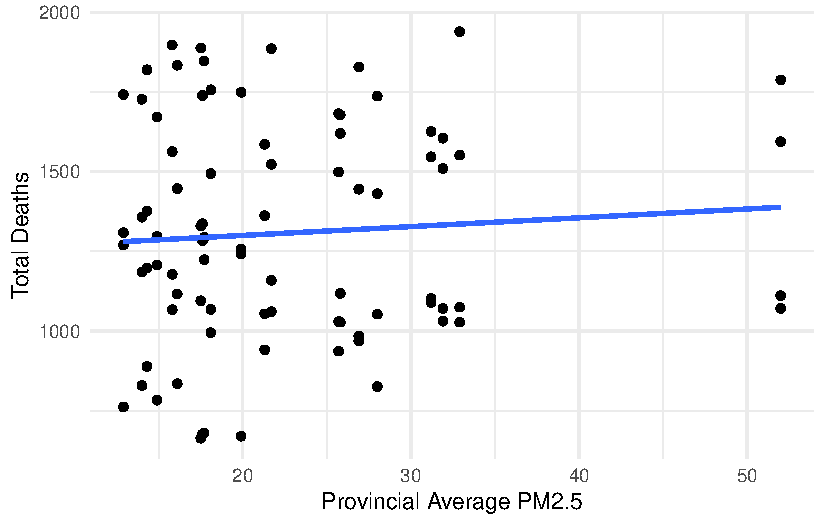
\includegraphics{paper_files/figure-pdf/fig-all-1.pdf}

}

\caption{\label{fig-all}Provincial Average PM2.5 Quantity Vs Total
Deaths}

\end{figure}%

\begin{figure}

\centering{

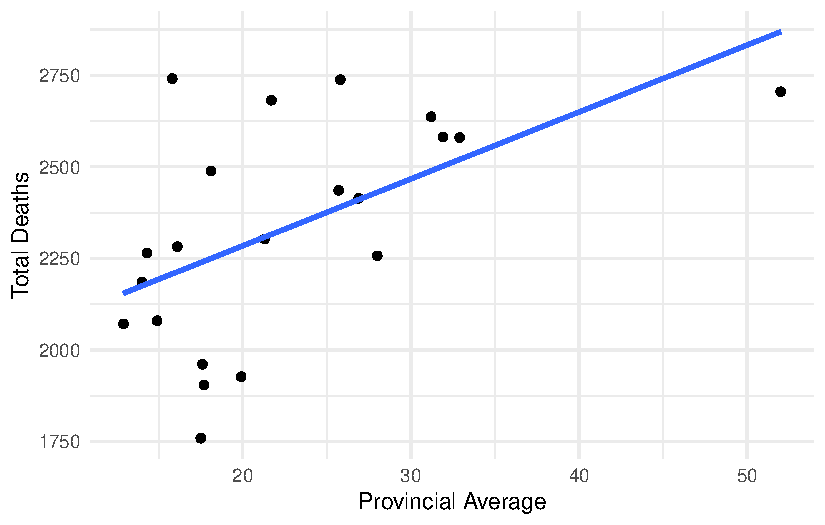
\includegraphics{paper_files/figure-pdf/fig-lung-1.pdf}

}

\caption{\label{fig-lung}Lung Related Causes Mortality Rates vs Average
PM2.5 Quantity}

\end{figure}%

\begin{figure}

\centering{

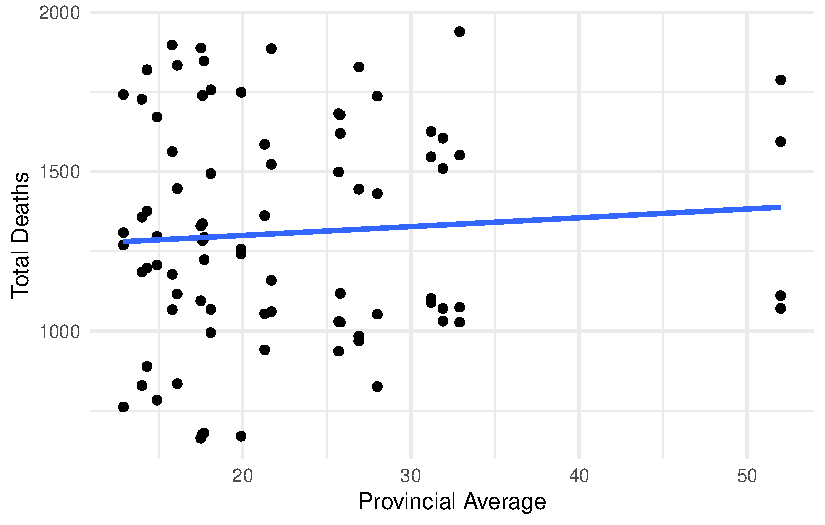
\includegraphics{paper_files/figure-pdf/fig-heart-1.pdf}

}

\caption{\label{fig-heart}Heart Related Causes Mortality Rates vs
Average PM2.5 Quantity}

\end{figure}%

Talk more about it.

And also planes (\textbf{?@fig-planes}). (You can change the height and
width, but don't worry about doing that until you have finished every
other aspect of the paper - Quarto will try to make it look nice and the
defaults usually work well once you have enough text.)

\begin{figure}

\centering{

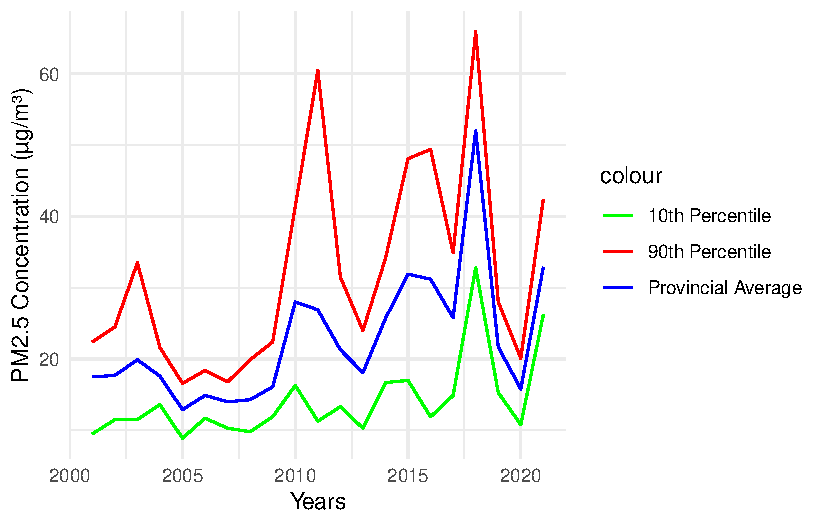
\includegraphics{paper_files/figure-pdf/fig-annual-1.pdf}

}

\caption{\label{fig-annual}Annual Trends of PM2.5 Concentrations in
Alberta}

\end{figure}%

\begin{figure}

\centering{

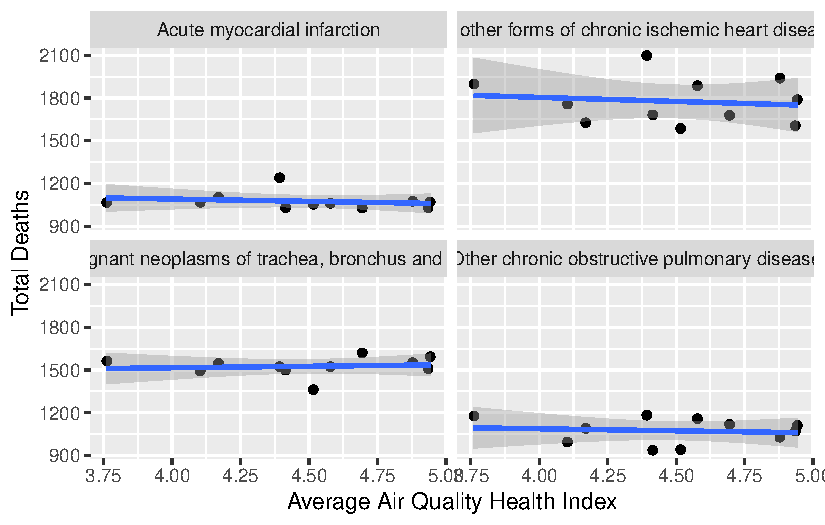
\includegraphics{paper_files/figure-pdf/fig-four-1.pdf}

}

\caption{\label{fig-four}Mortality Rates vs.~Air Quality Health Index}

\end{figure}%

\begin{figure}

\centering{

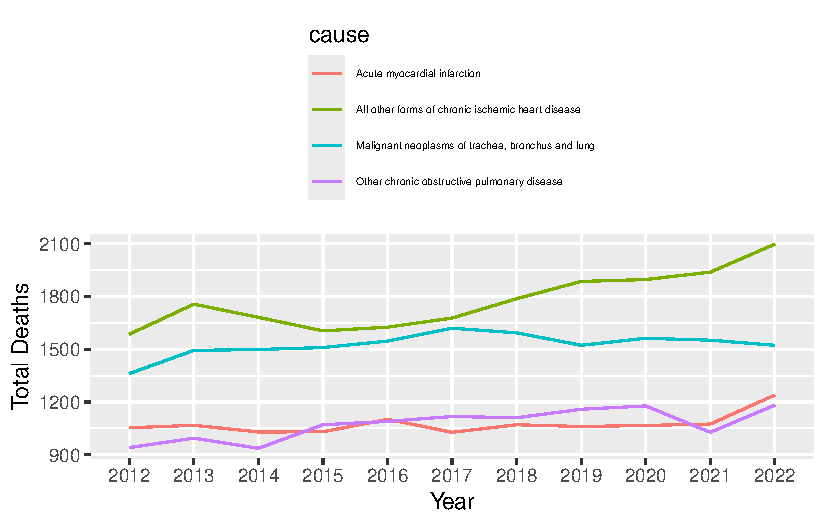
\includegraphics{paper_files/figure-pdf/fig-cause-1.pdf}

}

\caption{\label{fig-cause}Total Deaths by Year for Each Cause}

\end{figure}%

\begin{figure}

\centering{

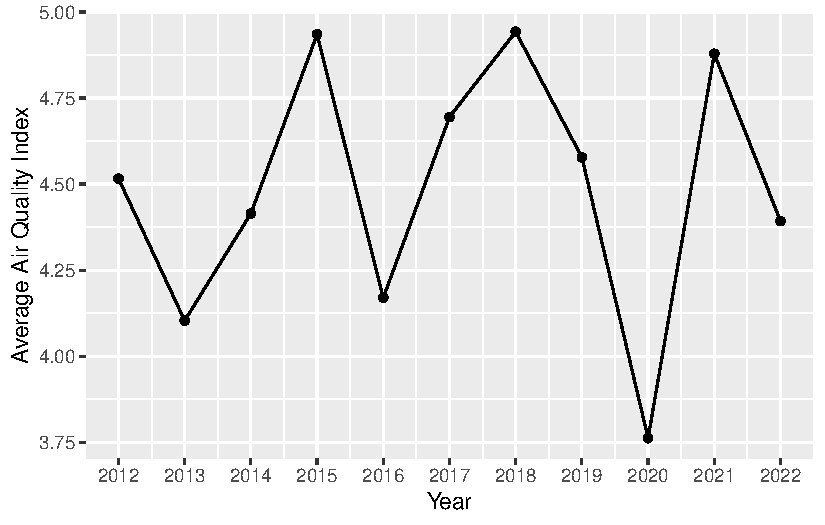
\includegraphics{paper_files/figure-pdf/fig-average_air-1.pdf}

}

\caption{\label{fig-average\_air}Average Air Quality Health Index by
Year}

\end{figure}%

Talk way more about it.

\section{Model}\label{model}

The goal of our modelling strategy is twofold. Firstly,\ldots{}

Here we briefly describe the Bayesian analysis model used to
investigate\ldots{} Background details and diagnostics are included in
Appendix~\ref{sec-model-details}.

\subsection{Model set-up}\label{model-set-up}

Define \(y_i\) as the number of seconds that the plane remained aloft.
Then \(\beta_i\) is the wing width and \(\gamma_i\) is the wing length,
both measured in millimeters.

\begin{align}
y_i | \mu_i, \phi &\sim \text{NegBin}(\mu_i, \phi) \\
\mu_i &= \exp(\alpha + \beta x_i) \\
\alpha &\sim \text{Normal}(0, 2.5) \\
\beta &\sim \text{Normal}(0, 2.5) \\
\phi &\sim \text{Exponential}(1)
\end{align}

We run the model in R (R Core Team 2023) using the \texttt{rstanarm}
package of (\textbf{rstanarm?}). We use the default priors from
\texttt{rstanarm}.

\subsubsection{Model justification}\label{model-justification}

We expect a positive relationship between the size of the wings and time
spent aloft. In particular\ldots{}

We can use maths by including latex between dollar signs, for instance
\(\theta\).

\section{Results}\label{results}

Our results are summarized in \textbf{?@tbl-modelresults}.

\begin{table}

\caption{\label{tbl-modelcauses}Different causes of mortality and their
death counts}

\centering{

\centering
\begin{tabular}[t]{lcc}
\toprule
  & Poisson & Negative binomial\\
\midrule
Ischemic Heart Disease & \num{0.510} & \num{0.510}\\
 &  & \vphantom{2} (\num{0.002})\\
Trachea/Bronchus/Lung Cancer & \num{0.353} & \num{0.353}\\
 &  & \vphantom{1} (\num{0.002})\\
COPD & \num{0.004} & \num{0.004}\\
 &  & (\num{0.002})\\
\midrule
Num.Obs. & \num{9048} & \num{9048}\\
Log.Lik. & \num{-69064.136} & \num{-53402.269}\\
ELPD & \num{-69078.6} & \num{-53405.5}\\
ELPD s.e. & \num{468.1} & \num{70.9}\\
LOOIC & \num{138157.2} & \num{106811.0}\\
LOOIC s.e. & \num{936.3} & \num{141.9}\\
WAIC & \num{138157.2} & \num{106811.0}\\
RMSE & \num{97.30} & \num{97.30}\\
\bottomrule
\end{tabular}

}

\end{table}%

\begin{table}

\caption{\label{tbl-modelheart}Heart related causes death count and the
air quality}

\centering{

\centering
\begin{tabular}[t]{lc}
\toprule
  & heart causes model\\
\midrule
(Intercept) & \num{8.02}\\
 & (\num{0.18})\\
provincial\_average & \num{0.00}\\
 & (\num{0.01})\\
\midrule
Num.Obs. & \num{21}\\
Log.Lik. & \num{-163.733}\\
ELPD & \num{-164.5}\\
ELPD s.e. & \num{0.5}\\
LOOIC & \num{329.0}\\
LOOIC s.e. & \num{1.0}\\
WAIC & \num{328.9}\\
RMSE & \num{142.90}\\
\bottomrule
\end{tabular}

}

\end{table}%

\begin{table}

\caption{\label{tbl-modellung}Lung related causes death count and the
air quality}

\centering{

\centering
\begin{tabular}[t]{lc}
\toprule
  & Lung Causes model\\
\midrule
(Intercept) & \num{7.57}\\
 & (\num{0.20})\\
provincial\_average & \num{0.01}\\
 & (\num{0.01})\\
\midrule
Num.Obs. & \num{21}\\
Log.Lik. & \num{-160.858}\\
ELPD & \num{-161.6}\\
ELPD s.e. & \num{0.8}\\
LOOIC & \num{323.3}\\
LOOIC s.e. & \num{1.6}\\
WAIC & \num{323.2}\\
RMSE & \num{248.30}\\
\bottomrule
\end{tabular}

}

\end{table}%

\section{Discussion}\label{discussion}

\subsection{First discussion point}\label{sec-first-point}

If my paper were 10 pages, then should be be at least 2.5 pages. The
discussion is a chance to show off what you know and what you learnt
from all this.

\subsection{Second discussion point}\label{second-discussion-point}

\subsection{Third discussion point}\label{third-discussion-point}

\subsection{Weaknesses and next steps}\label{weaknesses-and-next-steps}

Weaknesses and next steps should also be included.

\newpage

\appendix

\section*{Appendix}\label{appendix}
\addcontentsline{toc}{section}{Appendix}

\section{Additional data details}\label{additional-data-details}

\section{Model details}\label{sec-model-details}

\subsection{Posterior predictive
check}\label{posterior-predictive-check}

In \textbf{?@fig-ppcheckandposteriorvsprior-1} we implement a posterior
predictive check. This shows\ldots{}

In \textbf{?@fig-ppcheckandposteriorvsprior-2} we compare the posterior
with the prior. This shows\ldots{}

\begin{figure}

\begin{minipage}{0.50\linewidth}

\centering{

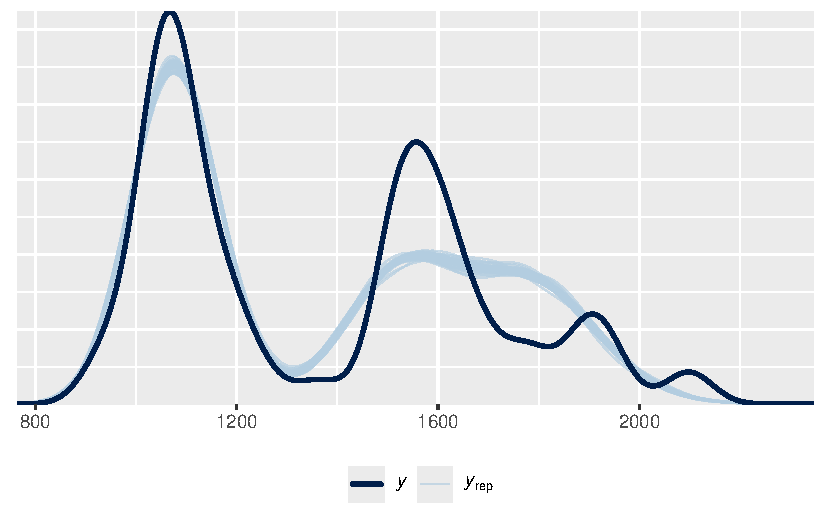
\includegraphics{paper_files/figure-pdf/fig-ppcheckfirst-1.pdf}

}

\subcaption{\label{fig-ppcheckfirst-1}Posterior prediction check}

\end{minipage}%
%
\begin{minipage}{0.50\linewidth}

\centering{

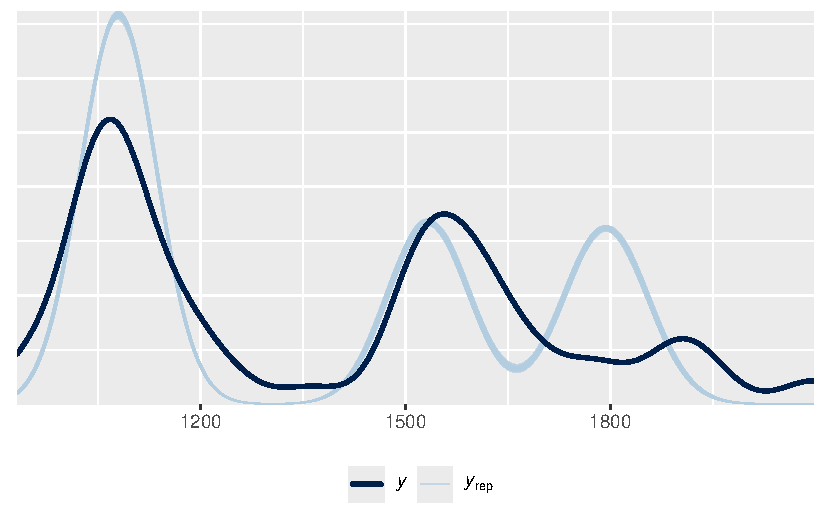
\includegraphics{paper_files/figure-pdf/fig-ppcheckfirst-2.pdf}

}

\subcaption{\label{fig-ppcheckfirst-2}Comparing the posterior with the
prior}

\end{minipage}%

\caption{\label{fig-ppcheckfirst}Examining how the model fits, and is
affected by, the data}

\end{figure}%

\begin{figure}

\begin{minipage}{0.50\linewidth}

\centering{

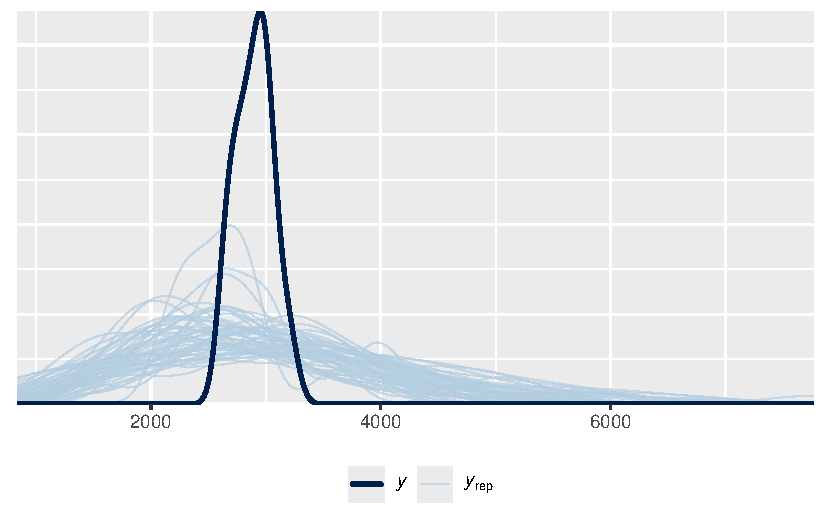
\includegraphics{paper_files/figure-pdf/fig-ppcheckheartlung-1.pdf}

}

\subcaption{\label{fig-ppcheckheartlung-1}Posterior prediction check}

\end{minipage}%
%
\begin{minipage}{0.50\linewidth}

\centering{

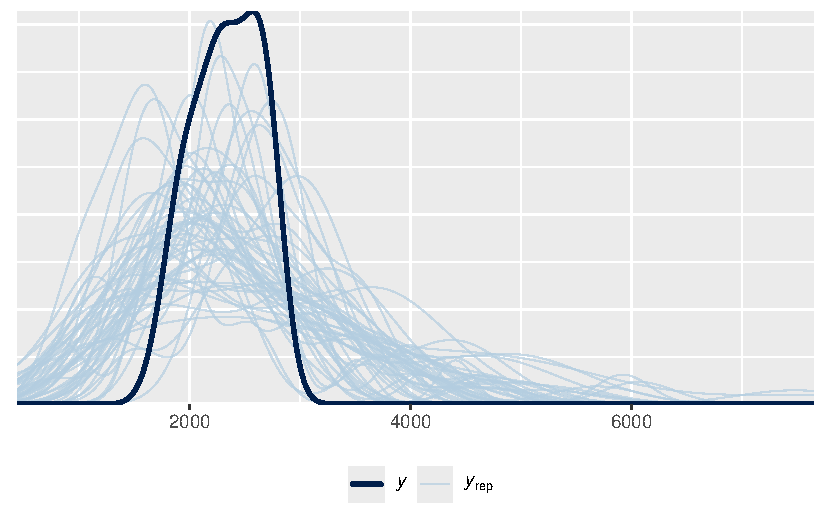
\includegraphics{paper_files/figure-pdf/fig-ppcheckheartlung-2.pdf}

}

\subcaption{\label{fig-ppcheckheartlung-2}Comparing the posterior with
the prior}

\end{minipage}%

\caption{\label{fig-ppcheckheartlung}Examining how the model fits, and
is affected by, the data}

\end{figure}%

\subsection{Diagnostics}\label{diagnostics}

Figure~\ref{fig-stanareyouokay-1} is a trace plot. It shows\ldots{} This
suggests\ldots{}

Figure~\ref{fig-stanareyouokay-2} is a Rhat plot. It shows\ldots{} This
suggests\ldots{}

\begin{figure}

\begin{minipage}{0.50\linewidth}

\centering{

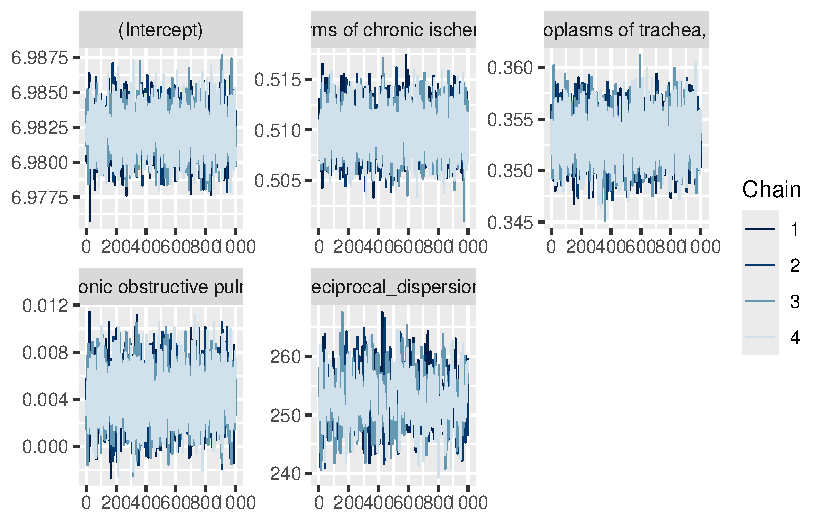
\includegraphics{paper_files/figure-pdf/fig-stanareyouokay-1.pdf}

}

\subcaption{\label{fig-stanareyouokay-1}Trace plot}

\end{minipage}%
%
\begin{minipage}{0.50\linewidth}

\centering{

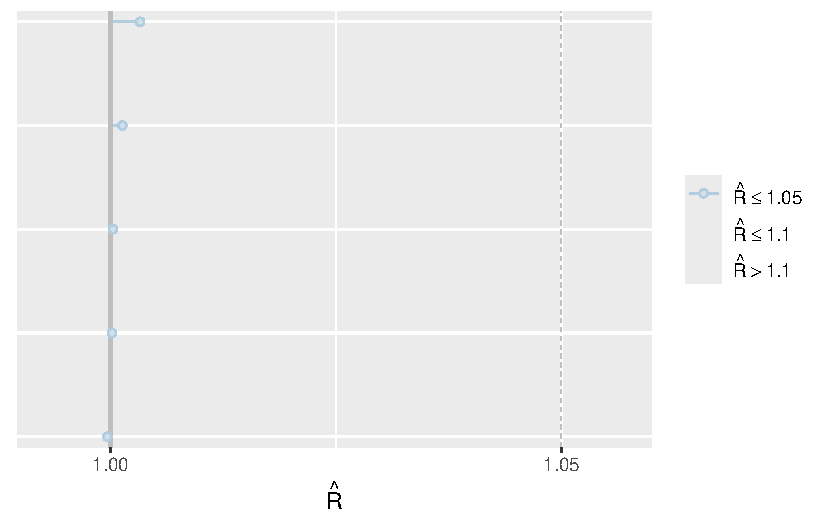
\includegraphics{paper_files/figure-pdf/fig-stanareyouokay-2.pdf}

}

\subcaption{\label{fig-stanareyouokay-2}Rhat plot}

\end{minipage}%
\newline
\begin{minipage}{0.50\linewidth}

\centering{

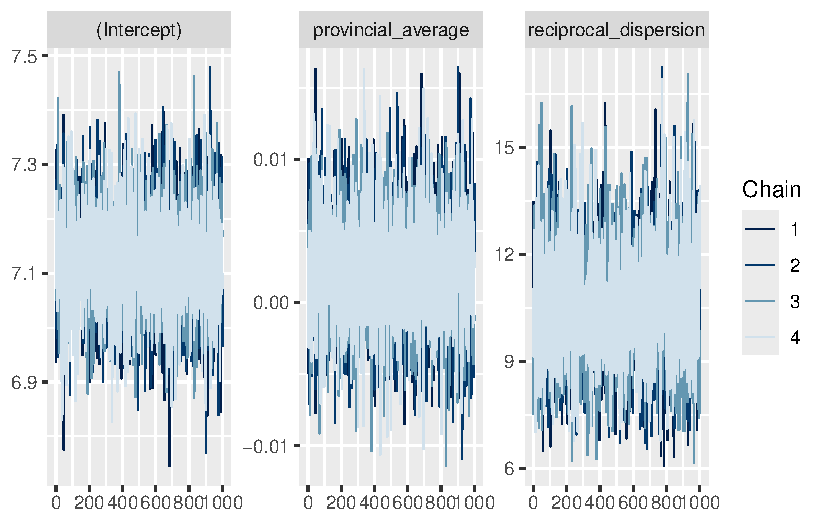
\includegraphics{paper_files/figure-pdf/fig-stanareyouokay-3.pdf}

}

\subcaption{\label{fig-stanareyouokay-3}Trace plot}

\end{minipage}%
%
\begin{minipage}{0.50\linewidth}

\centering{

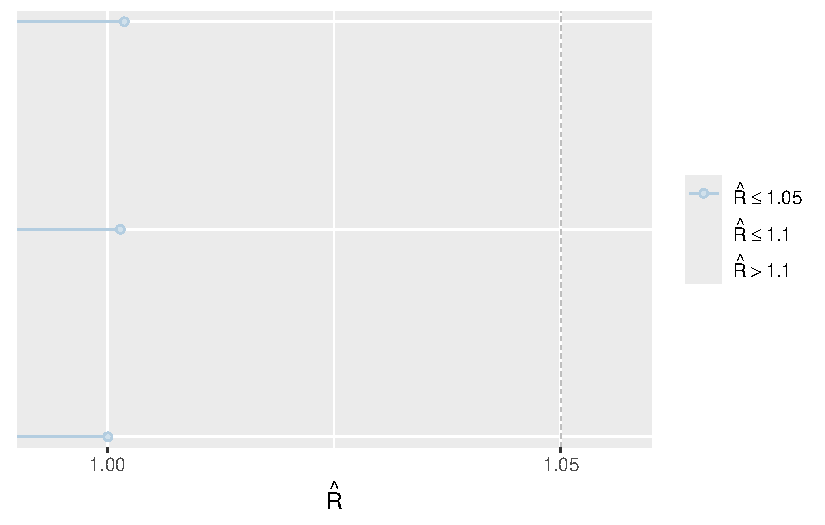
\includegraphics{paper_files/figure-pdf/fig-stanareyouokay-4.pdf}

}

\subcaption{\label{fig-stanareyouokay-4}Rhat plot}

\end{minipage}%

\caption{\label{fig-stanareyouokay}Checking the convergence of the MCMC
algorithm}

\end{figure}%

\newpage

\section*{References}\label{references}
\addcontentsline{toc}{section}{References}

\phantomsection\label{refs}
\begin{CSLReferences}{1}{0}
\bibitem[\citeproctext]{ref-pollution}
Alberta Government. 2023. {``Air Indicators -- Fine Particulate
Matter.''}
\url{https://www.alberta.ca/air-indicators-fine-particulate-matter}.

\bibitem[\citeproctext]{ref-model}
Arel-Bundock, Vincent. 2022. {``{modelsummary}: Data and Model Summaries
in {R}.''} \emph{Journal of Statistical Software} 103 (1): 1--23.
\url{https://doi.org/10.18637/jss.v103.i01}.

\bibitem[\citeproctext]{ref-pm}
Board, California Air Resources. 2024. {``Inhalable Particulate Matter
and Health (PM2.5 and PM10).''}
\url{https://ww2.arb.ca.gov/resources/inhalable-particulate-matter-and-health}.

\bibitem[\citeproctext]{ref-gg}
Clarke, Erik, Scott Sherrill-Mix, and Charlotte Dawson. 2023.
\emph{Ggbeeswarm: Categorical Scatter (Violin Point) Plots}.
\url{https://github.com/eclarke/ggbeeswarm}.

\bibitem[\citeproctext]{ref-report}
Environment, Ministry of, and Protected Areas. 2021. {``Status of Air
Quality in Alberta.''}
\url{https://open.alberta.ca/dataset/9b00aab3-c37d-4080-854e-5f329c621b92/resource/057c65ac-7837-49bb-9528-38c2611540c4/download/epa-alberta-air-zones-report-2019-2021.pdf}.

\bibitem[\citeproctext]{ref-jan}
Firke, Sam. 2023. \emph{Janitor: Simple Tools for Examining and Cleaning
Dirty Data}. \url{https://github.com/sfirke/janitor}.

\bibitem[\citeproctext]{ref-rstan}
Goodrich, Ben, Jonah Gabry, Imad Ali, and Sam Brilleman. 2022.
{``Rstanarm: {Bayesian} Applied Regression Modeling via {Stan}.''}
\url{https://mc-stan.org/rstanarm/}.

\bibitem[\citeproctext]{ref-air}
government, Alberta. 2023a. {``Air Quality Index by Municipality.''}
\url{https://open.alberta.ca/opendata/air-quality-index-by-municipality\#detailed}.

\bibitem[\citeproctext]{ref-deaths}
---------. 2023b. {``Leading Causes of Death.''}
\url{https://open.alberta.ca/opendata/leading-causes-of-death}.

\bibitem[\citeproctext]{ref-alberta}
---------. 2024. {``Alberta.''} \url{https://www.alberta.ca/}.

\bibitem[\citeproctext]{ref-ncbi}
Med, Lancet Respir. 2020. {``Prevalence and Attributable Health Burden
of Chronic Respiratory Diseases, 1990--2017: A Systematic Analysis for
the Global Burden of Disease Study 2017.''}
\url{https://www.ncbi.nlm.nih.gov/pmc/articles/PMC7284317/}.

\bibitem[\citeproctext]{ref-here}
Müller, Kirill. 2020. \emph{Here: A Simpler Way to Find Your Files}.
\url{https://here.r-lib.org/}.

\bibitem[\citeproctext]{ref-tib}
Müller, Kirill, and Hadley Wickham. 2023. \emph{Tibble: Simple Data
Frames}. \url{https://tibble.tidyverse.org/}.

\bibitem[\citeproctext]{ref-who}
Organization, World Health. 2024. {``Air Quality, Energy and Health.''}
\url{https://www.who.int/teams/environment-climate-change-and-health/air-quality-energy-and-health/health-impacts\#:~:text=The\%20main\%20pathway\%20of\%20exposure,and\%20ultimately\%20leading\%20to\%20disease}.

\bibitem[\citeproctext]{ref-citeR}
R Core Team. 2023. \emph{R: A Language and Environment for Statistical
Computing}. Vienna, Austria: R Foundation for Statistical Computing.
\url{https://www.R-project.org/}.

\bibitem[\citeproctext]{ref-repel}
Slowikowski, Kamil. 2024. \emph{Ggrepel: Automatically Position
Non-Overlapping Text Labels with 'Ggplot2'}.
\url{https://ggrepel.slowkow.com/}.

\bibitem[\citeproctext]{ref-mass}
Venables, W. N., and B. D. Ripley. 2002. \emph{Modern Applied Statistics
with s}. Fourth. New York: Springer.
\url{https://www.stats.ox.ac.uk/pub/MASS4/}.

\bibitem[\citeproctext]{ref-reshape}
Wickham, Hadley. 2007. {``Reshaping Data with the {reshape} Package.''}
\emph{Journal of Statistical Software} 21 (12): 1--20.
\url{http://www.jstatsoft.org/v21/i12/}.

\bibitem[\citeproctext]{ref-ggplot}
---------. 2016. \emph{Ggplot2: Elegant Graphics for Data Analysis}.
Springer-Verlag New York. \url{https://ggplot2.tidyverse.org}.

\bibitem[\citeproctext]{ref-tidy}
Wickham, Hadley, Mara Averick, Jennifer Bryan, Winston Chang, Lucy
D'Agostino McGowan, Romain François, Garrett Grolemund, et al. 2019b.
{``Welcome to the {tidyverse}.''} \emph{Journal of Open Source Software}
4 (43): 1686. \url{https://doi.org/10.21105/joss.01686}.

\bibitem[\citeproctext]{ref-rohan}
---------, et al. 2019a. {``Welcome to the {tidyverse}.''} \emph{Journal
of Open Source Software} 4 (43): 1686.
\url{https://doi.org/10.21105/joss.01686}.

\bibitem[\citeproctext]{ref-readxl}
Wickham, Hadley, and Jennifer Bryan. 2023. \emph{Readxl: Read Excel
Files}. \url{https://CRAN.R-project.org/package=readxl}.

\bibitem[\citeproctext]{ref-dp}
Wickham, Hadley, Romain François, Lionel Henry, Kirill Müller, and Davis
Vaughan. 2023. \emph{Dplyr: A Grammar of Data Manipulation}.
\url{https://dplyr.tidyverse.org}.

\bibitem[\citeproctext]{ref-read}
Wickham, Hadley, Jim Hester, and Jennifer Bryan. 2024. \emph{Readr: Read
Rectangular Text Data}. \url{https://readr.tidyverse.org}.

\bibitem[\citeproctext]{ref-knit}
Xie, Yihui. 2023. \emph{Knitr: A General-Purpose Package for Dynamic
Report Generation in r}. \url{https://yihui.org/knitr/}.

\bibitem[\citeproctext]{ref-kable}
Zhu, Hao. 2024. \emph{kableExtra: Construct Complex Table with 'Kable'
and Pipe Syntax}. \url{https://CRAN.R-project.org/package=kableExtra}.

\end{CSLReferences}



\end{document}
